% based on Msc dissertation template of University of Edinburgh

\documentclass[msc,deptreport, cs]{infthesis}
\usepackage{subfig, amsmath}
\usepackage{couriers}
\usepackage{float}
\usepackage{listings}
\usepackage[hyphens]{url}
\usepackage[hidelinks]{hyperref}
\graphicspath{{figures/}}
\tolerance=500
\newfloat{lstfloat}{htbp}{lop}
\floatname{lstfloat}{Listing}

\lstset{ 
  basicstyle=\linespread{1}\ttfamily, 
  frame=single,
}

\begin{document}
\begin{preliminary}

\title{Developing an Application \\to Introduce Parallel \\Task Scheduling}

\author{Juntong Liu}

\abstract{
}

\maketitle

\section*{Acknowledgements}
Any acknowledgements go here. 

\tableofcontents
\end{preliminary}


\chapter{Introduction}

Computing resource is in high demand both in industry and for academic research. In industry, companies are collecting terabytes or even petabytes of user data to provide customized services. Also, machine learning algorithms are widely used to provide suggestions and to extract information from media files. Processing these files and executing these algorithms all requires a huge amount of computing resource. In academic research, many researchers in subjects like hydromechanics and electrics rely on simulation to predict the performance of models. In this case, more computing resource is consumed for better resolution.

However, researchers said Moore's Law will not be effective in the near future (ref), meaning speed of improvement in single core performance may be far behind the increasing demand. Therefore, the typical way to utilize more computing resource is to use multiple processors to work on the same task in parallel. Traditional code for single core execution cannot be used directly for parallel execution. They have to be modified. One common solution to parallelize a big task is to divide it into small tasks that can be executed separately on multiple processors. However, in most of cases, the small tasks cannot be independent because they might require data produced by other tasks. The dependency can be usually represented by a DAG (directed acyclic graph) called task graph.

In large-scaled systems, tasks in a task graph are managed and scheduled to processors by a scheduler dynamically based on certain scheduling algorithm. To have better understanding of task graph scheduling, students need to learn the algorithms. However, learning such algorithms are not easy for many students for several reasons:

\begin{itemize}
  \item There are many models to describe the behavior of processors in real life. Students can be confused by the variety.
  \item Algorithms are usually given based on a certain model. For other models, there might be many variants that are slightly different, making things more confusing.
  \item Task scheduling requires predicting states of the cluster for a long duration. This is hard because it requires good imagination and detailed understanding of the behavior of models.
  \item Some algorithms requires sophisticated control over the timeline, or have a complex mathematical model which is hard to understand.
\end{itemize}

This project aims to develop a game-like application to help the students learn concepts in task graph scheduling, in addition to algorithms. For any schedule, it can simulate the execution timeline based on a variety of cluster configurations. It also provides a step to step tutorial to help students learn the mechanisms and algorithms. For tutors, this application can also be used for demonstration.

\chapter{Background}

\section{Task Graph Scheduling} \label{sec:comm}

The topic of this project is task graph scheduling. Figure \ref{fig:graph} shows an example of task graph. Each task graph contains several tasks, each labeled by its identifier and duration (in brackets). Arrows in the graph are used to describe dependencies by pointing from predecessor to successor. When there is dependency, the successor task have to be delayed until its predecessor is finished. For one task graph, there can be many different schedules, figure \ref{fig:schedule} shows one of which, based on the cluster with two processors, using lines with arrows to represent that the period is occupied by certain work. Execution of this task graph takes 23 time units for sequential execution. However, the total time is reduced to 14 units by separating the workloads to two processors.

\begin{figure}[!htb]
    \centering
    \vspace{1em}
    \subfloat[task graph]{ 
        \label{fig:graph}
        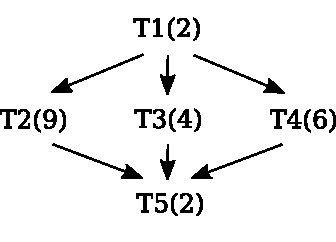
\includegraphics[width=0.3\columnwidth]{graph1.pdf}
    } \hspace{2em}
    \subfloat[schedule]{
        \label{fig:schedule}
        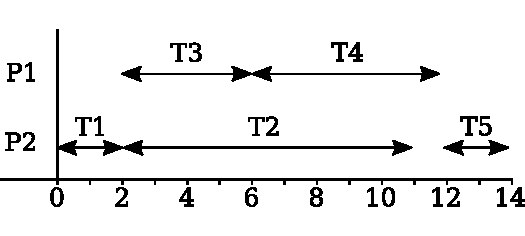
\includegraphics[width=0.45\columnwidth]{schedule1.pdf}
    }
    \caption{A example of task graph scheduling}
    \label{fig:example}
\end{figure}

When one task depends on another task, it usually means the successor requires data generated by the predecessor, which takes time to transfer between processors in reality. As a result, the successor task have to be delayed until all the data it depends on are received. To describe this behavior, communication cost is sometimes considered in the schedule. A very important feature is that it takes no time when the predecessor and successor are executed in the same processor, because the successor can easily utilize data cached locally without taking time to fetch it from other processors.

The execution of schedules can be described by many different models. A very simplified model can totally ignore the communication cost, which is used in in figure \ref{fig:example}. For such models, execution time of tasks can be easily described and estimated by mathematical expressions, by sacrificing accuracy of prediction. There are also models providing very detailed description of the behavior, based on clusters in real life. For these models, the mathematical expressions could be very complex, especially when considering competition of resources. Here are several well-developed variances of models:
\begin{itemize}
    \item \textbf{Heterogeneous vs.\ homogeneous performance:} For simplified models, processors in the cluster is usually assumed to be equally powerful. Such models are considered to describe homogeneous clusters. In real life, difference in processors is also common. Clusters consisting of different types of processors are called heterogeneous clusters (ref Topcuoglu). 
    \item \textbf{Practical vs.\ ideal (immediate) communication:} As described previously, communication cost can be totally ignored in ideal models. However, there are also many models used to describe the behavior of communication in real life. For example, the communication cost might depend on the size of messages (ref), or even state of shared resources in the cluster (ref Kwok1998).
    \item \textbf{Single vs.\ multiple communication channels:} The amount of communication channels is one of main difference when describing the communication behavior. For most devices connected the Internet, the primary limit is usually the total bandwidth. But for dedicated clusters, they are usually built on infrastructures with special optimizations for inter-cluster communications. In this case, processors might not suffer from performance loss when communicating with multiple processors.
\end{itemize}

\section{HLFET Algorithm}

There are many algorithms for task graph scheduling designed for different models. In this project, only BNP (bounded number of processors) scheduling algorithms for arbitrary task graph will be introduced. Among these algorithms, the HLFET algorithm will be used as the example because it is a simple and typical one of list scheduling algorithms, a group of widely used algorithms.

The core logic of list scheduling algorithms is to give priorities to tasks according to heuristic functions, then always execute tasks with higher priority as early as possible. It is called list scheduling because tasks are usually sorted into a list based on the priority, and tasks are always taken from the top of the list. In HLFET, priority of tasks is defined as the longest path to exit. In other words, for any path from one task to any exit within the task graph, the priority of this task is defined as the maximum sum of durations for tasks on the path. Following this method, tasks on the critical path are usually given higher priorities. Communication cost is ignored in this algorithm because it is designed for ideal communication model.

Take the task graph in figure \ref{fig:graph} as example. Using $P(Tn)$ for the priority for task Tn and $T(Tn)$ for duration of task Tn, priorities of tasks are given as follows:
\begin{align*}
P(T5) &= T(T5) = 2\\
P(T2) &= T(T2) + P(T5) = 2 + 9 = 11\\
P(T3) &= T(T3) + P(P5) = 2 + 4 = 6\\
P(T4) &= T(T4) + P(T5) = 2 + 6 = 8\\
P(T1) &= T(T1) \max(P(T2), P(T3), P(T4)) = 2 + 11 = 13
\end{align*}

Using the priorities, the tasks are sorted as: T1, T2, T4, T3, T5. Following the strategy described previously, figure \ref{fig:schedule1-2} shows one possible schedule made by HL. One thing to be noticed is HLFET does not explicitly define the behavior if the start time of one task on multiple processors are the same, when trying to execute this task as soon as possible. In this case, HLFET could generate multiple possible schedules.

\begin{figure}[!htb]
  \centering
  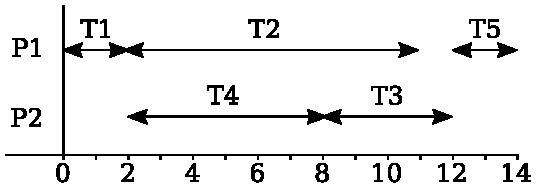
\includegraphics[width=0.45\columnwidth]{schedule1-2.pdf}
  \caption{A possible schedule generated by HLFET}
  \label{fig:schedule1-2}
\end{figure}

\chapter{Design}

\section{Learning Experience}

\subsection{Game Modes}

Similar to games, this application is divided into many levels. Each level can have different game mode for different purposes:

\begin{itemize}
  \item \textbf{Static mode:} In this mode, students are given several task graphs and a cluster. Students can create schedules by scheduling tasks in task graphs to processors in the cluster. When one schedule is created, it can be executed to generate the timeline, so that the student can improve the schedule according to the execution timeline. Each level can have several target times. When all the tasks are finished, the performance of the schedule will be evaluated according to the targets.
  
  The main purpose of this mode is to let the students analyze and optimize schedules. The target times in these levels are usually very tight and the graphs are usually designed to emphasize the usage of certain optimization techniques. By attempting such levels, the understanding of related techniques can be reinforced.

  \item \textbf{Dynamic mode:} Different from static mode, the state of the cluster will be simulated in real time. After the start of game, several task graphs will be revealed at certain time point. The student is required to schedule the tasks to processors when the simulation is running. Similar to static mode, the time cost to finish all the tasks will be recorded and the performance will be evaluated based on target times.
  
  Compared to static mode, this mode is designed to be more competitive to provide more challenges to students. When playing these levels, student have to analyze task graphs quickly and make schedules immediately. To have better performance, the student need to extract the main characteristics of tasks graphs given, rather than analyzing them using mathematical models, which improves the proficiency of students when using certain techniques. Also, since it generates more pressure and requires less mathematical analysis, it might seems more like a game and more enjoyable for some students.

  \item \textbf{Tutorial mode:} Levels in this mode are usually developed based on static mode. For tutorial levels, some help text will be displayed describe concepts, operations and algorithms. A tutorial can operate on the game engine freely. By listening to operations made by the student, tutorials can be made into an interactive process to help students learn faster. Levels in this mode are usually made educational only. Students can find detailed description of techniques that are required when playing other levels.

  \item \textbf{Sandbox mode:} This mode is also developed based on static mode. The user can create games by selecting clusters and task graphs, then play the the created game freely. This mode also provides several standard algorithms, so that the user can try these algorithms to check the scheduling result. This mode can be helpful for demonstration and testing because the user can build any scenarios according to requirements, in addition to check and compare the behavior of algorithms in such scenarios.
\end{itemize}

\subsection{Design of Interface} \label{sec:interface}

The design of game interface is given in figure \ref{fig:layout}. The main aim of the design is to make it clear and simple. Therefore, most of information related to the game is given inside one window. The layout is separated to two main areas. The top area shows the current state of the game, including the cluster and the task graphs. On the left hand side, it shows the state of processors inside the cluster. On the right hand side, the space is taken by task graphs. A high proportion of the window is given to task graphs because there are many detailed information for each task graph and there could be even multiple task graphs within one game. The bottom area, consisting of two rails, handles most of interactions with the user. The first rail shows the queue of tasks scheduled to processors, while the second rail shows the execution timeline when the game is running.

\begin{figure}[!htb]
  \centering
  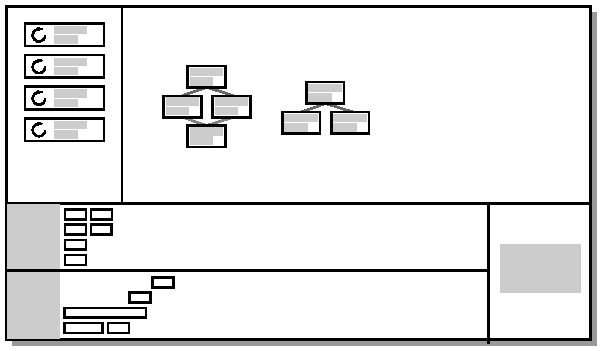
\includegraphics[width=0.8\columnwidth]{layout.pdf}
  \caption{Design of interface}
  \label{fig:layout}
\end{figure}

Two main interactions in this application is hovering and drag \& drop. Hovering is mainly used for following purposes:

\begin{itemize}
  \item \textbf{Revealing internal connection:} Since most of content inside the interface is tightly coupled, when mouse is hovered over any element, all related elements will be highlighted, which allows the user to discover the internal relationships easily without getting confused. For example, when hovering over any task in task graphs, the position inside task queue, the duration of execution inside timeline and the processor executed the task will all be highlighted. Taking a common operation in the game, scheduling the successor task to the same processor as the predecessor, as example, the user can find the processor the predecessor is scheduled to easily by hovering over the predecessor in the task graph.
  \item \textbf{Providing extra details:} Since the layout is designed very compact, some details cannot be displayed inside the window. Such information can be rendered when hovering over certain elements. For example, speedups for each processor is rendered only when hovering over the processor and size of communication will only be rendered when hovering over related tasks.
\end{itemize}

Drag \& drop is used mainly to edit the schedule. The user can schedule one task to one processor by dragging the task from task graph, then drop it inside the task queue. In addition, tasks inside the task queue can also be moved to edit the schedule.

The base resolution of the window is decided to be 1440x720, to make it suitable for most of screens. For a window with limited resolution, number of processors and size of task graphs have to be limited, if they are required to be always visible. After changing the layout several times, the clusters are limited to have no more than 4 processors and the task graphs are required to be no larger than 4x4. According to experience in design of levels, clusters and task graphs in such size is sufficient to construct very complex scenarios, if the purpose of the scenarios is to let humans to make the schedule manually.

\section{Execution Logic}

An elementary feature of this application is to execute the schedule and show the result of execution. For ideal communication models, the execution can be easily predicted by mathematical expressions, but for models considering cost of communication, the execution is hard to predict. The main reason is that schedules of tasks usually do not specify execution of communications. For one schedule, using different order or delay of communications can easily generate different execution timelines in models with limited communication resource. 

The difference is usually related to competition of resource: when some workloads are prioritized, some will be delayed. For example, when one processor establishes a communication channel with another processor, it also consumes communication bandwidth in the cluster, making other communication affected. In following sections, such difference in execution and related competition of resource will be described as ``conflicts'', where rules are applied to provide a determined result. But before the conflicts, communication models will be introduced first.

\subsection{Communication Models}

As is described in section \ref{sec:comm}, one difficulty in task graph scheduling is variety of communication models. To reflect the variety, four different communication models are selected as follows:

\begin{enumerate}
  \item \textbf{Ideal (immediate) communication (IC):} Communication does not cost any time. Tasks will only be delayed if any of its dependency is not finished.
  \item \textbf{Background communication with multiple channels (BCMC):} One processor can communicate with unlimited amount of processors in both directions. The only limit is one processor can only have one channel sending to another processor, meaning no more than one communication block can be sent from one processor to another at any time. The limit is made since bandwidth of one connection is always limited in real life, although there could be multiple connections.
  \item \label{sec:bcsc} \textbf{Background communication with single channel (BCSC):} One processor can send to or receive from only one processor at any time. Instead of having multiple connections, this model describes processors with single connection, and the total bandwidth is limited. Therefore, one communication in progress can occupy the entire bandwidth, making other communications blocked.
  \item \textbf{Synchronous (blocked) communication (SC):} One processor cannot execute tasks and communicate with other processors at the same time. Also, it allows only one channel in one direction like described in mode \ref{sec:bcsc}. This model describes the scenario when using synchronous communication libraries like Java IO or MPI synchronous mode in single thread.
\end{enumerate}

\subsection{First Conflict and Rule 1}

With more strict communication models, there can be more conflicts. One option is to let the student decide how to solve the conflicts, but sometimes it makes the learning experience too detailed and annoying, so the program have to add more rules as tie breaking strategies to simplify the process in such cases.

\begin{figure}[!htb]
  \centering
  \vspace{1em}
  \hspace{3em}
  \subfloat[task graph]{ 
      \label{fig:conflict1-1}
      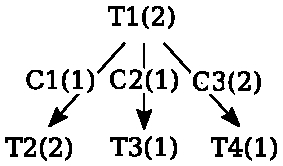
\includegraphics[width=0.25\columnwidth]{graph2.pdf}
  } \hspace{4em}
  \subfloat[timeline 1]{
      \label{fig:conflict1-2}
      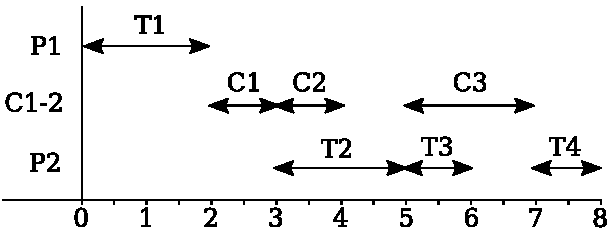
\includegraphics[width=0.48\columnwidth]{schedule2-1.pdf}
  } \\
  \subfloat[timeline 2]{
      \label{fig:conflict1-3}
      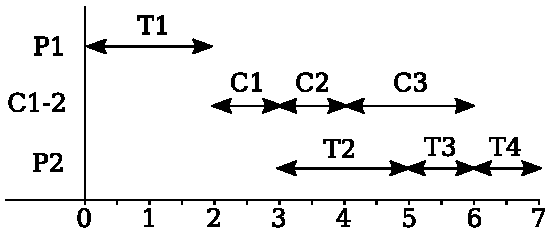
\includegraphics[width=0.44\columnwidth]{schedule2-2.pdf}
  } \hspace{1em}
  \subfloat[timeline 3]{
      \label{fig:conflict1-4}
      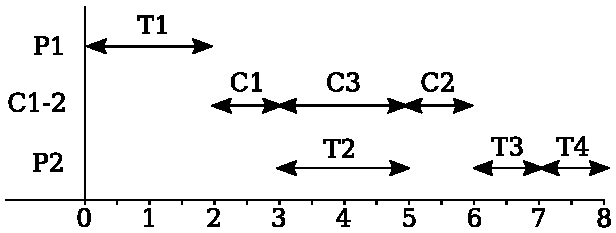
\includegraphics[width=0.48\columnwidth]{schedule2-3.pdf}
  }
  \caption{One task graph and possible timelines to demonstrate effect of communication order in non-ideal models}
  \label{fig:conflict1}
\end{figure}

In all non-ideal modes, one conflict is when two tasks scheduled on one processor relies on data from another processor, because two data packages have to be sent in certain order. The strategy used is to allow communication required by one task only when it is the first task in the schedule (rule 1). In other words, communication required by one task will be delayed if there is any task ahead of it in the schedule. Figure \ref{fig:conflict1} shows one example task graph and three possible execution timelines if T1 is scheduled to processor 1 (P1) and remaining tasks are scheduled to processor 2 (P2). For the task graph, tasks are labeled as ``Tn(Duration)'' and communications are labeled as ``Cn(Duration)''.

As shown in the timelines, for one given schedule, there could be many results if the order and time of tasks are not explicitly specified. However, according to "rule 1", the execution result will always be timeline 1. Although other strategies can provide better performance like in timeline 2 (also known as early fetch), this rule is chosen for its reliability, simplicity, and less uncertainty. Another option is to leave the decision to students. However, there are two problems: 1) It have to be decided based on very precise estimation of execution, which might be too challenging for a student, even for many algorithms; 2) It will make the interface very complex because it requires precise control of time.

\subsection{Second Conflict}

Another conflict happens only for single channel models, which is the order of communication for one task. Figure \ref{fig:conflict2} shows an example of the conflict. For task graph given in \ref{fig:conflict2-1}, by scheduling T1 to P1, T2 to P2 and T3 to P3, even when rule 1 is applied, there are still multiple possible execution results, which are shown in figure \ref{fig:conflict2-2} and \ref{fig:conflict2-3}. 

\begin{figure}[!htb]
  \centering
  \vspace{1em}
  \hspace{3em}
  \subfloat[task graph]{ 
      \label{fig:conflict2-1}
      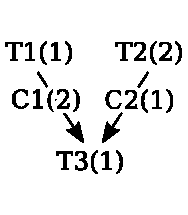
\includegraphics[width=0.18\columnwidth]{graph3.pdf}
  } \hspace{4em}
  \subfloat[timeline 1]{
      \label{fig:conflict2-2}
      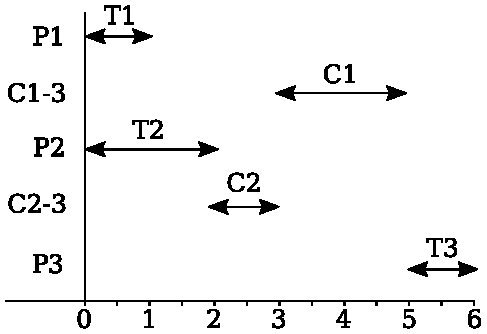
\includegraphics[width=0.4\columnwidth]{schedule3-1.pdf}
  } \\
  \subfloat[timeline 2]{
      \label{fig:conflict2-3}
      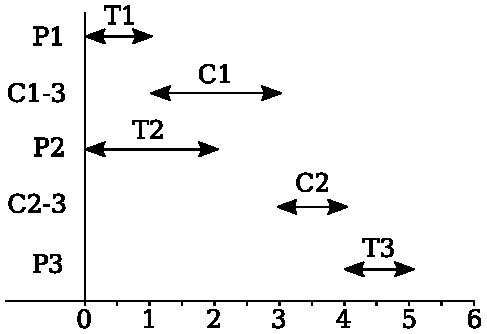
\includegraphics[width=0.4\columnwidth]{schedule3-2.pdf}
  } \hspace{1em}
  \subfloat[timeline 3]{
      \label{fig:conflict2-4}
      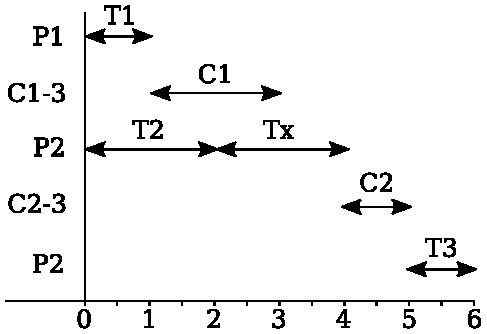
\includegraphics[width=0.4\columnwidth]{schedule3-3.pdf}
  }
  \caption{One task graph and possible timelines to demonstrate effect of communication order in single channel models}
  \label{fig:conflict2}
\end{figure}

The main problem is the order of communications that T3 depends on. When C1 is executed first, the result is figure \ref{fig:conflict2-2} and when C2 is executed first, it generates figure \ref{fig:conflict2-3}. A straight forward solution is to always attempt to receive the data that is available earlier, which is C1 in this case, similar to greedy strategies. According to the figure, it provides better performance indeed. However, in some other cases, when another task Tx is assigned to P2, assuming synchronous communication model, C2 can be terribly delayed.

According to the timelines, it seems changing the order of communication can have significant effect over execution of other tasks, especially when the resources are limited. Therefore, the decision is left to the student. In multiple communication models, since there is no such conflict, the system will handle communication automatically, while in single communication models, the student have to decide the order manually. However, it does not mean tasks being executed can be paused to execute communications. When one task have been under execution, communications will be delayed until execution finishes.

\subsection{Third Conflict and Rule 2} \label{sec:rule2}

In synchronous communication model, there is also conflict between execution of tasks and communication. Figure \ref{fig:conflict3} shows an example of the conflict when T2 is scheduled to P2, and remaining tasks are scheduled to P1. When T1 finishes, there are two options: communicate with P1 first (figure \ref{fig:conflict3-2}), or execute T3 first (figure \ref{fig:conflict3-3}).

\begin{figure}[!htb]
  \centering
  \subfloat[task graph]{ 
      \label{fig:conflict3-1}
      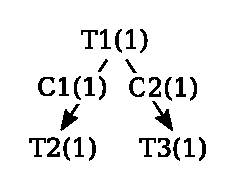
\includegraphics[width=0.22\columnwidth]{graph4.pdf}
  } \hspace{1em}
  \subfloat[timeline 1]{
      \label{fig:conflict3-2}
      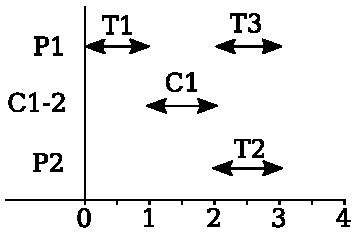
\includegraphics[width=0.3\columnwidth]{schedule4-1.pdf}
  } \hspace{1em}
  \subfloat[timeline 2]{
      \label{fig:conflict3-3}
      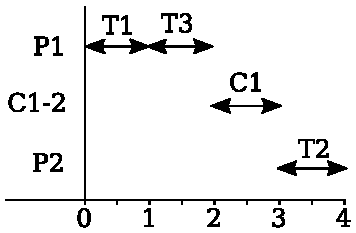
\includegraphics[width=0.3\columnwidth]{schedule4-2.pdf}
  }
  \caption{One task graph and possible timelines to demonstrate conflict between execution and communication in synchronous communication model}
  \label{fig:conflict3}
\end{figure}

As can be observed in figures, if processors are allowed to execute next task before communication, it is possible to block other processors for a long time, when there are many connected tasks. To remove unnecessary delay caused by this conflict, the choice is to force processors communicate before executing tasks (rule 2). Under this rule, the result execution will always be figure \ref{fig:conflict3-2}.

\subsection{Other Conflicts and Behavior} \label{sec:conflict}

There are still many conflicts that are not mentioned. For example, figure \ref{fig:conflict4} shows two possible execution results for the task graph given in figure \ref{fig:conflict4-1} when scheduling T1 to P1, T2 to P2 and T3 to P3. However, since such conflicts do not happen as frequent as previously described ones, and the effect to general performance is negligible in most of cases, the behavior is not explicitly defined. Also, defining too much rules for details also brings more complexity for students to learn. Instead, the behavior when such conflicts happen depends on the implementation of simulation engine. The detailed execution will be described in section \ref{sec:simulation}.

\begin{figure}[!htb]
  \centering
  \subfloat[task graph]{ 
      \label{fig:conflict4-1}
      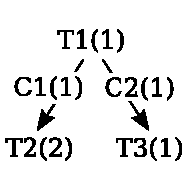
\includegraphics[width=0.18\columnwidth]{graph5.pdf}
  } \hspace{0.5em}
  \subfloat[timeline 1]{
      \label{fig:conflict4-2}
      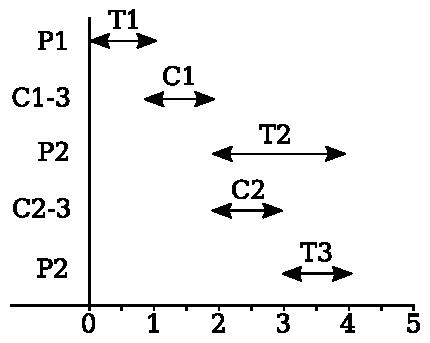
\includegraphics[width=0.34\columnwidth]{schedule5-1.pdf}
  } \hspace{0.5em}
  \subfloat[timeline 2]{
      \label{fig:conflict4-3}
      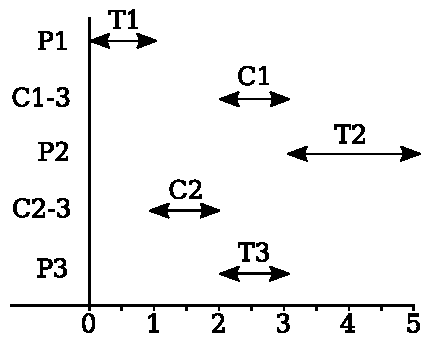
\includegraphics[width=0.34\columnwidth]{schedule5-2.pdf}
  }
  \caption{One task graph and possible timelines to demonstrate effect of different output order in single communication models}
  \label{fig:conflict4}
\end{figure}

To summarize, for conflicts stated in previous sections, when any of them exists in one model, the related rule will always be applied, otherwise the student will be required to decide the behavior. More precisely, the first conflict appears in BCMC, BCSC and SC models, so rule 1 will be applied. The second conflict appears in BCSC and SC models, so the student have to decide the behavior manually. The third conflict happens in SC models, so rule 2 will be applied. For other unstated conflicts, the behavior will depend on the implementation.

\section{Platform and Libraries}

\subsection{Programming Language}

This project is designed to be a cross-platform desktop application. While C++ is the typical choice for such requirements, Java is chosen as the main language in development. 

The biggest difficulty of using C++ is compilation on different platforms. For example, programs on Windows are usually compiled against all DLLs (dynamically linked libraries) selected and provided by the developer and distributed with all its dependencies bundled. However on Linux, programs are usually compiled against SOs (shared objects) provided by system, then distributed as source file or single binary file. Such difference brings complexity in compilation and potential issues in distribution.

Oppositely, compilation of Java file is much easier. With help of virtual machine, compiled binary files can be executed on different platforms without any extra step. Since Java executable files are usually packed in Jar files, distribution is also convenient.

\subsection{GUI Library} \label{sec:opengl}

As is said in previous sections, the interface is designed to be interactive, which means the application will heavily rely on operations like hovering and drag \& drop. Also, it requires rendering overlays and transparency frequently. For widgets based traditional GUI frameworks, these operations usually requires usage of complex or low level APIs, which brings difficulty in development and potential compatibility issues. Therefore, games are usually developed based on dedicated GUI frameworks.

GUI frameworks used in games are usually built on low level libraries like DirectX and OpenGL. One reason is they are usually directly connected to hardware operations, which saves much performance in rendering complex shapes. Another reason is these libraries allows GUI frameworks developed in immediate mode, making it easier to develop highly dynamic scenes. Compared to retained mode, the developer do not need to refresh windows manually in immediate mode because every frame is refreshed and rendered separately.

OpenGL is chosen as the rendering library for its cross-platform availability and simplicity. Although OpenGL do not provide APIs in Java, there are several libraries in Java providing the bridge. Among these libraries, LWJGL 3 is chosen for several reasons:

\begin{itemize}
  \vspace{-1em}\item It includes bridges to several convenient native libraries like STB and GLFW.
  \vspace{-1em}\item It has very good documents and community support.
  \vspace{-1em}\item It provides full exposure of OpenGL APIs.
  \vspace{-1em}\item It it up-to-date.
\end{itemize}

With help of LWJGL, programs written in Java can still easily access native libraries, while there is no need to have special compilation steps for different platforms because the dependencies are already included and handled by LWJGL.

\chapter{Implementation}

\section{General Architecture}

The core part of this project follows the widely used MVC (model-view-controller) architecture. View classes include \verb+Window+, \verb+Page+ and \verb+Widget+. Model classes include \verb+Cluster+, \verb+Graph+ (for task graphs) and \verb+Schedule+. \verb+Game+ objects work as the controller. Compared to typical implementations of MVC, modules in this project is more flexible and coupled. For example, for some simple interfaces, user input can be handled directly within the view object (\verb+Page+), without using external controllers.


\begin{figure}[!htb] 
  \centering
  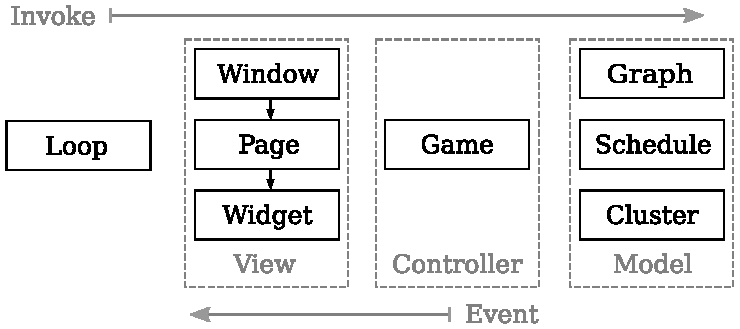
\includegraphics[width=0.65\columnwidth]{architecture.pdf} \vspace{-0.3em}
  \caption{Architecture of application}
  \label{fig:architecture}
\end{figure} \vspace{-0.5em}

Since the GUI framework is built based on low level APIs, the main loop of the program have to be explicitly created. The main loop provides the basic ticking mechanism, driving all the underlying layers following the structure in figure \ref{fig:architecture}: The \verb+Window+ object checks user input at every tick, and refreshes the frame based on a fixed interval. Inside every refresh operation, the ticking call will be distributed to all the \verb+Pages+ and \verb+Widgets+. When some special widgets are refreshed, the ticking call will be passed to the game engine. Based on another interval, the state of game will be updated.

Other operations are also passed between modules following the same structure: Modules on the right hand side is responsible to operate according to instructions from modules on the left hand side. One main reason is references in this project are usually held in single direction to keep the structure clean. However, there are some scenarios that modules on the right hand side need to notify modules on the left hand side. For example, the controller will let the view to show statistics when the game is finished. Such operations are implemented based on the event system described in section \ref{sec:event}. Using the event bus, events can be broadcast globally without reference of certain objects.

\section{Simulation Engine}

\subsection{Choice of Execution Method}

There are mainly two ways to predict the execution results: calculate the timeline based on mathematical relationships (calculation), or simulate the execution process, then record the states (simulation). Assume this question: predict how much time does it take to execute one task that takes 2 seconds, on a processor with 2x speed. For calculation methods, the only thing required is calculate $2\div 2 = 1$ second. On the other hand, here is an example for simulation methods. First cut the time into ticks, for example 20 ticks per second. Therefore, tasks that takes 2 seconds is equivalent to 40 ``work packages''. Secondly, calculate how much work can be done within one tick. For a processor with 2x speed, it is 2 ``work packages'' per tick. The final step is to keep execute ticks until finished work on the processor reaches 20 ``work packages''. By calculating difference in tick count, which is 20 ticks in this case, it can be concluded the execution takes 1 second.

It seems calculation methods are much simpler and efficient, but the simulation method is used for several reasons:

\begin{itemize}
  \item It's hard to find a generic expression for different scenarios in calculation methods. For example, in ideal communication model, for one task, the earliest start time is maximum of the finish times of all its dependencies and processor's earliest available time. While for BCMC model, the finish times of dependencies will be changed to finish time added by communication time, if the tasks are executed on different processors. For similar reasons, the expression will be very complex for some communication models. However for simulation, the developer only need to describe the actual behavior of one processor, according to requirements of the communication model, which is usually called transition functions. Therefore, changing in communication models is equivalent to changing the transition function, which is significantly easier to implement and validate.
  \item The execution uses tasks as unit, rather than time in calculation models. In other words, the tasks are atomic. For example, when one task is executed by calculation, it takes the entire period in the timeline immediately. Because of this nature, the developer have to check the states of all related processors in the entire period for conflicts. Also, the execution order of tasks have to be carefully arranged for correct behavior. Although this problem can be resolved by always executing tasks scheduled to the earliest available processor, for tasks with communications, it will become very complicated because workloads are tightly coupled and shared by processors.
  \item Simulation models are more suitable for animations. This application is required to ``run'' a schedule. When cursor on the timeline moves, simulation models are actually running the tick under the cursor. Therefore, the animated execution is actually rendering the history of simulation engine in real time. However for calculation modes, extra steps are required to "make up" the animated execution.
\end{itemize}

\subsection{Execution of Simulation} \label{sec:simulation}

The simulation engine is constructed based on a model close to clusters in real life. It maintains a list of processors, each keeping an input buffer, a list of active communication channels, a task being executed and an output buffer, although the output buffer is not stored explicitly inside processor objects for global visibility.

When simulation is running, it follows a very simple logic: keep executing ticks until there is nothing to be executed on all processors. One tick has three phases, listed as follows:

\begin{enumerate}
  \item \verb+tickPre1+: Every processor checks task queue to prepare for next task to execute. If next task requires communication with other processors, establish communication channel with target processor.
  \item \verb+tickPre2+: If the processor is available and all dependencies are met, fetch the task from task queue and prepare for execution.
  \item \verb+tickPost+: Execute communications and task by updating the progress. If communication or task is finished, update the state of processor and buffers accordingly.
\end{enumerate}

One tick is separated into 3 phases for two reasons:

\begin{itemize}
  \item As required by rule 2 described in section \ref{sec:rule2}, communications will always be executed first if there is conflict between communication and execution of tasks. Therefore, in the first phase, all processors will check for communications and allocate resource for it. When resource is occupied by communication in some communication models, task will not be fetched in the second phase, thus ensures higher priority for communications. The two phases cannot be merged because there is usually coupling between processors. For example, assuming the two phases are merged, if processor A is ticked first and it fetches one task with no dependency, processor B, the later ticked, cannot establish communication channel with processor A because resource in processor A is already occupied, which violates rule 2.
  \item Between phase 2 and phase 3, the state is written to history. The basic concept is processors only decides what to do in one tick inside the two pre-tick phases, while no execution is performed, making the end of phase 2 suitable to record the state. If phase 2 and 3 are merged and history is updated at phase 3, one apparent consequence is that execution of tasks taking only 1 tick will never be recorded because the execution is finished inside the tick. Actually, the result is execution of every task will miss 1 tick in history. There is work-around for this problem, but to keep the states clean, phase 2 and phase 3 are kept separated.
\end{itemize}

Within one phase, all processors in the cluster will be traversed, following the order given in layout described in section \ref{sec:format}. When there is potential competition of resource, execution will always follow the "first come first served" logic. Taking the conflict described in section \ref{sec:conflict}, if P2 is positioned before P3 in layout, the timeline in figure \ref{fig:conflict4-2} will always happen, because P2 is ticked earlier in first pre-tick and it occupies the communication channel before P3 attempts to. Oppositely, if P3 is positioned before P2, the timeline in section \ref{fig:conflict4-3} will always happen.

\subsection{Float Error Handling}

The progresses of all communications and executions of tasks are stored as double-precision float numbers, because the base speed and speedups of processors are allowed to be float numbers, using 0 for started and 1 for finished. When using float numbers in simulations, the developer need to be careful with the error. For example, if a processor completes 20\% of the task (0.2 out of 1), when 5 ticks are completed, the progress might not be 1. The value is usually a number slightly smaller or larger than 1 because 0.2 cannot be precisely represented by float numbers.

The solution is to have an acceptable margin of error. For example, consider $1 - 10^{-5}$ to be finished. However, the margin have to be decided carefully. If the margin too small, the value could easily fall outside the range. While if the margin is too large, which is larger than the difference generated by one iteration, the value can be considered finished before reaching the theoretical amount of iterations.

There is no ideal value for the margin. For longer tasks that takes more iterations to finish, the difference in one iteration is smaller, while the accumulated error is larger. The typical value of error $\epsilon$ is about $10^{-16} \sim 10^{-15}$ when using double-precision floats. For a task that requires n iterations, the difference of one iteration is $1/n$ and the accumulated error is $n\epsilon$. To achieve a balance, $\epsilon_0 = \sqrt{\epsilon} \approx 10^{-8}$ is used as the margin of error. In this case, the simulation will have error of 1 iteration for tasks taking over $10^7$ ticks, which is equivalent to over 30 hours, assuming 80 tick per second. Since tasks in this program usually takes only several seconds, the accuracy seems acceptable.

\section{GUI Framework and Interfaces}

The design of interface discussed in section \ref{sec:interface} requires the GUI framework to be very flexible. However, most of traditional GUI frameworks, when implementing advanced user interactions, introduces extra difficulty, since they are designed for traditional interfaces. Also, a high proportion of the design uses customized widgets. In this case, although traditional GUI frameworks usually provides a variety of built-in widget types, it doesn't provide much help. Therefore, the final choice is to implement a dedicated GUI framework based on OpenGL, as described in section \ref{sec:opengl}.

Development based on low level GUI frameworks is different from the experience using traditional GUI frameworks. For every widgets, the developer have to handle mouse events, check the bounding box and render the elements manually. It seems unnecessarily complex when implementing traditional interfaces, but when creating customized widgets, it provides very detailed control and exposure of low level APIs.

In addition to widgets, the implement of framework also takes much effort. In this project, GLFW is used to create windows and handle user inputs. From the developer's perspective, it provides only OpenGL contexts that can be rendered to, and global user inputs, like keyboard button state, mouse movement and mouse button state, based on coordinate system corresponding to the window's position. Therefore, for a framework, it have to work as a compatibility layer to provide decent abstraction of such APIs. For example, it have to align the rendering space to pixel based coordination, and to translate mouse events into interactions like click or drag. However, since this is not the focus of this project, many details will be skipped.

\subsection{Rendering Method}

Most of rendering in this project uses the painting system, based on OpenGL. Compared to hardware related APIs provided by OpenGL, this system provides much convenient operations like rendering shapes, characters and textures, using coordinates aligned to pixels.

\begin{figure}[!htb]
  \centering
  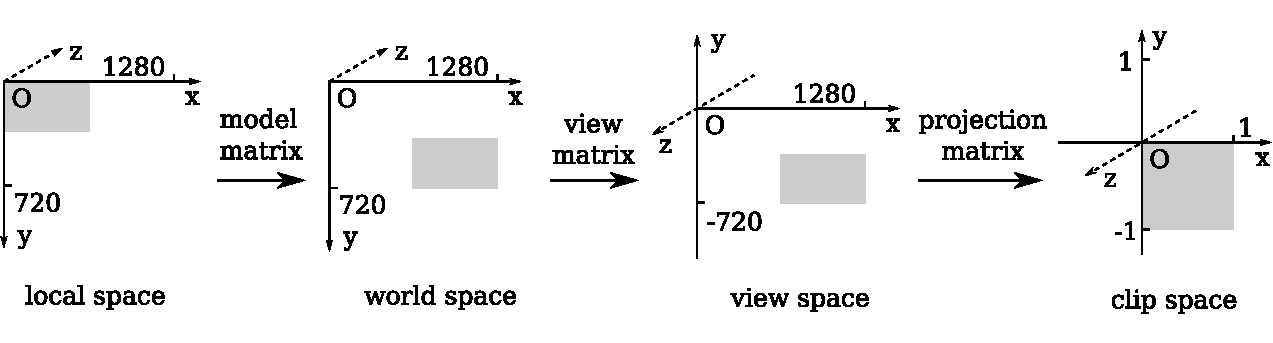
\includegraphics[width=\columnwidth]{matrix.pdf}
  \caption{Transformation matrixes and spaces}
  \label{fig:matrix}
\end{figure}

When developing 2D interfaces, the most intuitive coordination system is pixels. However, since OpenGL is designed for 3D rendering, all rendering instructions are positioned by a special coordinate system. In traditional 3D rendering, several matrixes are used to control the position of rendering. All the matrixes are modified for rendering in 2D space, as is shown in figure \ref{fig:matrix}. In this example, one rectangle with size of 640x360 is rendered to a window with size of 1280x720, shifted by 640 pixels in x direction and 360 pixels in y direction. In other words, by painting a 640x360 rectangle at point (0, 0), one square $x\in[0, 1]$, $y\in[-1, 0]$ should be actually rendered in clip space, since the entire window is equivalent to $x\in[-1, 1]$, $y\in[-1, 1]$ in clip space.

The coordination of rectangle is first transformed by model matrix to shift the rendering. Afterwards, it is transformed by view matrix into view space. In this step, view matrix describes the camera in this scene, then transfer the world coordination into relative coordination corresponding to the camera. Finally, projection matrix is used to transform the view space into clip space according to OpenGL specifications. In this program, view matrix will always describe a camera looking into the plane in the opposite direction of z-axis, and projection matrix will always transform $x\in[0, width]$, $y\in[-height, 0]$ into $x\in[-1, 1]$, $y\in[-1, 1]$. The model matrix is more flexible. Since model matrix can be used to shift all the rendering instructions, most of widgets relies on it to move inside the window.

To provide better control of shifting, model matrixes are kept as a stack, similar to \verb+glPushMatrix+ and \verb+glPopMatrix+ in fixed pipeline used in older versions of OpelGL(ref). Based on this system, shifting can be applied and restored multiple times. When the painting is shifted twice to (1, 1), it actually results in a shift to (2, 2). This is very helpful when rendering widgets inside containers because widget containers are required to provide shifting of child widgets and to be suitable for nested design.

To render in 2D space, another modification to OpenGL is that depth test is disabled. The design of OpenGL focuses on rendering in 3D space, where surfaces in the front will cover surfaces in the back, where depth test is used to ensure this behavior. When depth test is disabled, shapes rendered later will always cover shapes rendered earlier, which is more intuitive in 2D rendering.

\subsection{Widgets and Layout}

Widgets are most basic components in the interface. Since many customized widgets will be developed in this project, the interface of widgets are kept very simple. For all the widgets, they only need to implement these functions: 
\begin{itemize}
  \item Handle basic user input like mouse move, click, drag, drop and keyboard press.
  \vspace{-1em}\item Draw the content to the screen.
  \vspace{-1em}\item Refresh before rendering of every frame.
  \vspace{-1em}\item Clean up (for example, listeners) when it is removed.
\end{itemize}

Not every widget need to refresh the content or clean up the resources, but to implement advanced widgets, such functions can be helpful. For example, the widget rendering history of execution need to refresh the content whenever the engine is running. Also, for the widgets listening to events, it is convenient if they are allowed to cancel the listeners registered to the event bus when they are removed, otherwise there might be unexpected event handling and memory leak.

The layout is mainly controlled by widget containers (\verb+WContainer+) and pages. Widgets are uniquely positioned by its upper left corner and widget containers are used for the control, as is described in previous section. Figure \ref{fig:container} shows an example of nested containers. In this example, W2 and W3 are containers. W2 is a child of W3 and W1 is a chile of W2.
For children inside containers, vector V1 and V2 are used to describe the offset. When W2 is moved by modifying V1, V2 do not change, making W2 and all its children integrated when moved around.

\begin{figure}[!htb]
  \centering
  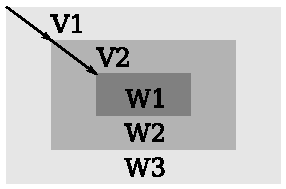
\includegraphics[width=0.26\columnwidth]{container.pdf}
  \caption{An example of nested widget containers}
  \label{fig:container}
\end{figure}

Pages are advanced version of widget containers, with an extra function to refresh the layout. Whenever the window is resized, this function will be called so the widgets inside the page will be moved according to the new size. There is no dynamic layout in this project, all the widgets are positioned by calculating the offset manually. Since there are not many pages in this project, creating layout manually seems acceptable. 

\section{Data Driven Format} \label{sec:format}

All the graphs, clusters and levels are data driven in this project, to provide convenience when creating games. Using JSON files, everyone can add extra levels without modifying the code.

\begin{lstfloat}
  \lstinputlisting{listings/cluster.json}
  \caption{Example of cluster in JSON}
  \vspace{-1em}
\end{lstfloat}

\begin{lstfloat}
  \lstinputlisting{listings/game.json}
  \caption{Example of game in JSON}
  \vspace{-1em}
\end{lstfloat}

\begin{lstfloat}
  \lstinputlisting{listings/graph.json}
  \caption{Example of graph in JSON}
  \vspace{-1em}
\end{lstfloat}

\begin{lstfloat}
  \lstinputlisting{listings/levels.json}
  \caption{Example of levels in JSON}
  \vspace{-1em}
\end{lstfloat}

\section{Algorithms and Estimator}

\section{Event System} \label{sec:event}

\subsection{Tutorials}

\chapter{Summary of Final System}

\section{Compilation and Distribution}

\section{Game Flow}

\subsection{Appearance and Components}

\subsection{Tutorial Levels}

\subsection{Game Levels}

\subsection{Sandbox Mode}

\chapter{Evaluation}

\section{User Testing}

\section{Code Quality}

\chapter{Conclusion}

\section{Future Suggestions} 

% Non exclusive communication

\section{Final Comments}

\bibliographystyle{plain}
\bibliography{main}

\end{document}
